\documentclass[10pt]{article}  % [12pt] option for the benefit of aging markers
\usepackage{amssymb,amsthm}    % amssymb package contains more mathematical symbols
\usepackage{graphicx}          % graphicx package enables you to paste in graphics
\usepackage[toc,page]{appendix}
\usepackage{listings}
\usepackage{color}
%%%%%%%%%%%%%%%%%%%%%%%%%%%%%%%%%
%
%    Page size commands.  Don't worry about these
%
\setlength{\textheight}{220mm}
\setlength{\topmargin}{-10mm}
\setlength{\textwidth}{150mm}
\setlength{\oddsidemargin}{0mm}

\definecolor{dkgreen}{rgb}{0,0.6,0}
\definecolor{gray}{rgb}{0.5,0.5,0.5}
\definecolor{mauve}{rgb}{0.58,0,0.82}

\lstset{frame=tb,
  language=Java,
  aboveskip=3mm,
  belowskip=3mm,
  showstringspaces=false,
  columns=flexible,
  basicstyle={\small\ttfamily},
  numbers=none,
  numberstyle=\tiny\color{gray},
  keywordstyle=\color{blue},
  commentstyle=\color{dkgreen},
  stringstyle=\color{mauve},
  breaklines=false,
  breakatwhitespace=true,
  tabsize=3
}

%%%%%%%%%%%%%%%%%%%%%%%%%%%%%%%%%%%%%%%%%%%%%%%%%%%%%%%%%%%%%%%
%
%    Definitions of environments for theorems etc.
%
\newtheorem{theorem}{Theorem}[section]          % Theorems numbered within sections - eg Theorem 2.1 in Section 2.
\newtheorem{corollary}[theorem]{Corollary}      % Corollaries etc. will be counted as Theorems for numbering
\newtheorem{lemma}[theorem]{Lemma}              % eg Lemma 3.1, ... Theorem 3.2, ... Corollary 3.3.
\newtheorem{proposition}[theorem]{Proposition}
\newtheorem{conjecture}[theorem]{Conjecture}

\theoremstyle{definition}
\newtheorem{definition}[theorem]{Definition}

\theoremstyle{remark}
\newtheorem{remark}[theorem]{Remark}
\newtheorem{example}[theorem]{Example} 

%%%%%%%%%%%%%%%%%%%%%%%%%%%%%%%%%%%%%%%%%%%%%%%
%
%        Preamble material specific to your essay
%
\title{CI346 Coursework}
\author{Chris Howell\\}

\begin{document}
\maketitle
 \begin{center}
  
\includegraphics{link.png}
  \end{center}
\newpage                     % optional page break
\begin{abstract}

A review into implicit and explicit concurrency with reference to a benchmark program written in Java.



\end{abstract}

\newpage                     % optional page break
\tableofcontents

\newpage                     % optional page break
\section{Part 1}\label{s:intro}
%
% The \label command is optional, but useful.  To cross-refer to a section/theorem/equation etc.
% labelled by \label{key}, use \ref{key}.  For example: Equation (\ref{eq:key}) follows from Theorem \ref{th:key}.


 \begin{center}
  \end{center}

\subsection{Concurrency}\label{ss:back}



Concurrency is a major issue when writing computer programs. Highly concurrent applications execute multiple aspects of the program simultaneously. While this approach does allow for the creation of complex programs with multiple components executing at the same time, this can also cause issues that are hard to reason about and identify the cause of.\\

Concurrency is often confused with parallelism, with this due to the illusion that concurrent applications give of processes executing at the same time. It should be noted that concurrency is multiple processes being executing sequentially at a fast pace to give the illusion that the process are executing at the same time, while parallelism executes the processes at the same time.\\

An example of a highly concurrent program would be an operating system. An operating system is highly concurrent as it needs to execute multiple aspects of the operating system in rapid succession, with this being achieved by a scheduling policy that allocates CPU time to each running process.\\

When using an operating system a good scheduling policy is essential because the user needs to believe the illusion that all the components are that they currently have running are executing at the same time. For example, a user reading their emails while listening to a music player should not be able to tell that these tasks are operation at different times.\\

For example, one common issue caused by concurrency is one thread accessing data that is currently being mutated by a separate thread. Because the data is in the process of being mutated by one thread, when the second thread attempts to also mutate the data unexpected results often occur. This can lead to unexpected program behaviour.\\

To counter these problems programming languages implement different approaches to ensuring that concurrently executing threads do not cause issues with other threads that are executing. For example, functional programming languages such as Haskell have no mutable state. By creating pure functions, functions that only manipulate variables that are local to them, many of the concurrency issues encountered in imperative programming languages simply do not occur. Imperative programming language such as Java would require a drastic overhaul to remove all mutable data, although it should be noted that Java does support immutable state via the use of final.\\

One common issue that arises from the use of concurrency is deadlock. Deadlock typically occurs when two process are competing for limited resources. An example of this would be when process A is waiting for process B to finish, while process B is also waiting for process A to finish.\\

Another common concurrency related issue that arises from the use of concurrency in programs is thread starvation. Thread starvation occurs when one process is taking up all the CPU times while another thread is waiting to be schedule CPU time. An example of thread starvation occurring would be in a GUI when the users presses a button, with nothing happens for a noticeable amount of time and then finally the button event occurs. It should be noted that thread starvation is a possible side effect of using synchronized methods, with this occurring when one thread holds onto a synchronized method for an unusual length of time. \\


\subsection{Explicit}\label{ss:back}


Explicit concurrency is defined by the developer, with this being achieved using threads in Java and C++.   Java allows the developer to explicitly define concurrent aspects of a program via the use of threads. The developer can define a new thread and then override the run method to enable them to define some behaviour to be executed by the thread.\\

Some of the advantages of using explicit concurrency are that CPU time can be better allocated resulting in less time unused and more time executing work. Applications that implement explicit concurrency efficiently have high performance.\\ 

Multiple threads can be defined in a program to execute concurrently[\ref{thread}]. One issue that arises from this approach is that as the size of the application grows it can be harder for the developer to reason about how the concurrent aspects of the program need to execute.\\

When a developer uses explicit concurrency they have to take care to ensure that issues such as deadlock are avoided. One way of achieving this in Java is by implemented synchronized methods. Only one thread can access a synchronized method at any given time. While the current executing thread has controlled of a synchronized method, no other thread can access the same method. This approach reduces the likelihood of shared data being mutated in an unexpected way. One issue that does occur from this approach is thread starvation.\\

Another approach to avoiding explicit concurrent issues is by declaring a variable final. By declaring a variable to be final it is no longer mutable. This means that threads are capable of retrieving this value, but unable to mutate it to cause unexpected results.\\

One useful approach to thread-based concurrency that a developer can take is the creation of a thread pool. By creating a thread pool the developer has a better degree of control over how multiple threads are created and executed. By combining thread creation with a loop the developer can create multiple threads without having to explicitly create and run each thread.\\

The alternative to a thread pool is a thread executor. The thread executor handles the creation and lifespan of the thread and allows the developer to set the number of threads to create. This is a useful feature as it lets you scale the amount of threads created depending on the number of cores that the current machine has available. By dynamically generating the number of threads created the developer can stop a concurrent program with overwhelming the CPU with a higher number of threads and tasks to execute.\\

One of the alternatives Java provides to using thread-based concurrency is via the use of future tasks and callable. They allow the developer to define a worker that implements callable so that it must return a value. This approach is arguably better that using raw threads because it creates code that is less blocking when return values are required\cite{O_F}. \\ 

Implementing a thread pool with futures and callable allows the developer the ability to create concurrent operations that execute in parallel. It is by no means required to use futures and callable with a thread pool as the developer is capable of using threads to execute some task in parallel.\\

While explicit concurrency is a useful tool for the developer it often requires a large amount of code to achieve the required the results. The developer is also forced to consider global state and how to effectively mutate variables without causing concurrency related issues.


\subsection{Implicit}\label{ss:back}

Implicit concurrency differs from explicit in that the programming language compiler  handles concurrently executing activities. Generally, when a program features implicitly concurrent processes executing, the developer states what activity they want to concurrently execute and then leaves the lower-level aspects of how to execute the activity up to the compiler/interpreter to handle.\\

Java 8 is the most recent iteration of Java and implements implicit concurrency into the language via the use of parallel streams. By using parallel streams, a developer can let the compile decide how best to implement the concurrent operations. A parallel stream has a built in sort function for common types, but can also be passed a custom comparator when required.\\

It should be noted that to truly utilize parallelism the tasks being completed must be appropriate. For example, attempting to sort using a parallel stream is less effective than checking if each number in an array is a prime number. The reason for this is because check if a number is prime in an array doesn't require any other data from the array than the number at that position being checked, with this meaning a parallel stream can rapidly iterate the array checking each number.\\

 For sorting, the parallel stream must  firstly break down the array into smaller sections, then sort these sections, put each of these sections back together and then finally sort the entire array again, with this being a time consuming process with little benefit.\\

One advantage of using implicit concurrency is that the developer spends less time worrying about how best to implement the concurrency and more on the functionality the program is intended to implement. For example, the parallel test created for this assignment contains significantly less code than then the explicit and thread pool tests.\\

Looking at the test class that implemented a parallel stream, the option they provide the developer is the use of concurrency while focusing on the logic. Apart from the setting up of the test environment for the test, almost the entire logic, along with the use of the parallel stream for parallelism are contained in a a few lines of code. \\

One disadvantage of using implicit concurrency is that arguably implicit doesn't have the same level of performance as explicitly defined concurrency\cite{O_P}. When a developer chooses to use explicit concurrency over implicit, they can then define exactly how they want the concurrent processes to operate. A highly skilled developer could potentially write a program with explicit concurrency that performs better than implicit.\\
\newpage

\section{Part 2}\label{s:intro}

\subsection{Performance test}\label{ss:back}

The tests were first executed a number of times before a sample was taken to calculate the average length of time each test took to run. This approach was to ensure the most accurate results could be obtained. \\

The benchmark application was tested across two different machines with varying levels of hardware, with the most noticeable between the two devices being their respective processors as this is most relevant for the performance tests.\\

The first device tested on was a home desktop computer that contained an over clocked Intel I5-2500K processor running at approximately 3.9GHz. The second device was laptop computer containing an AMD Dual-Core E-300 with a clock speed of approximately 1.3 GHz.\\

The tests were design to implement different implementation of concurrency and parallelism in Java. The tests each count the amount of prime number contained inside a randomly generated list. The first set of tests counted the amount of prime numbers contained in a list with one hundred million numbers, while the second contained one hundred thousand numbers. These tests where then repeated on a second machine.\\

Firstly, with the differences between the clock speed of the two processors selected, and the number of cores available to each of the processors, the tests performed on each of the machines were always going to highlight the drastic differences in performances between these two chips.\\

The benchmark program runs four tests of varying implementation and calculate then prints the time in seconds it took for each test to complete.  Each test implements the prime interface to use the default method to check if a number is prime, if so the counter is incremented. The total number of prime numbers found are printed along with the amount of time each test took. The number of prime numbers found are printed by each test to ensure consistency across the test results.\\  

\subsubsection{Intel I5-2500K}

As was expected all test results were shorter on the Intel machine[\ref{ibt1}] as the processor is more capable than the alternative test machines processor[\ref{abt1}]. \\

The first element that should be noted from the test results is that the implementation of explicit was the slowest, with the non concurrent class slightly faster. It should be noted that with variations in the test result times occasionally they swapped position as slowest test. \\

One reason that the class implementing raw threads is scoring approximately the same as non concurrent is that the implementation is a costly one[\ref{thread}]. By breaking the array into two separate arrays and then counting the number of prime number contained in each array sequentially is not a very efficient implementation of concurrency. It requires the first thread to have finished its calculations before starting the second thread and the second to have finished before adding the count of each array's prime numbers.\\

More interestingly is the results for the fastest benchmark test. Although using the thread pool was the second highest scoring test, the fastest test results came from using a parallel stream. This could be in part to the chosen test case, in this instance count the prime numbers, being well suited for parallel calculation. To test this prediction the amount of numbers being check was reduced from 100 million to 100 thousand.\\

After lowering the amount of numbers to check for each array, the tests were run again a number of times and the average calculated. The test results for the second test on the same machine are in stark contrast to the first batch of test results. After lowering the input data, and then using the parallel stream for counting prime numbers was the slowest performing test, with using raw threads being only slightly faster. This highlights the overhead required for setting up concurrent and parallel operations. For some operations it is simply not efficient to utilize a parallel stream or attempt to implement concurrency into a small problem. Both concurrent and parallel operations are at their most effective when the task to complete is \\


\subsubsection{AMD Dual-Core E-300}

As expected when using a machine with a process that features less cores and a lower clock speed, this has a direct impact on the amount of time each test took to execute. Each of the tests on this machine took significantly longer to complete their operations. Similarly to the tests run on the alternative test machine, the parallel stream test and thread pool test were the fastest executing tests.\\

One interesting aspect of the second test results is that the test featuring no concurrency executed the fasted.





\newpage
\section{Part 3}\label{s:intro}

C++ and Java are both object oriented programming languages that share a number of similarities syntactically, with each including common iteration techniques like loops, but these similarities are mostly superficial and when looking a little deeper at how they operator you can see that they are actually very different programming languages. While they are both considered object-oriented programming languages they differ in how they implement the object-oriented principles.\\

It should be noted that neither language is considered a true object-oriented programming language, but out of the two languages Java is considered the purer implementation of the object-oriented principles.\\

C++ is a language built on top of the C language with the aim of allowing the developer to create highly concurrent applications such as operating systems. With this aim in mind the language had to give developers greater control over how memory is management than a language like Java.\\ 

In comparison to this Java was also created to be a highly concurrent language, that featured a class based approach to object oriented principles. The key difference with Java is the approach to port ability. Java was created to work across a wide variety of devices regardless of hardware and operating system, as long as the device is capable of running the JVM, then it is capable of executing some Java code. 

\subsection{Concurrency}\label{ss:back}

Both Java and C++ are programming languages that feature concurrent libraries. Both languages allows the developer to create threads to execute concurrent aspects of a program. Unfortunately both C++ and Java feature mutable state which means implement concurrency into an application can also cause concurrency related issue such as deadlock and thread starvation.\\

Java allows a developer to implement synchronized methods to counter the issues caused by mutable state. By implementing a synchronized method, the developer can be sure that only one thread can access that method at any given time. This approach allows for greater reasoning about how the thread will manipulate data and reduce unexpected data manipulation from occurring. In the example[\ref{refSync}] an array is passed to a class containing only synchronized methods. While any thread can read the array, only one thread is capable of adding data at any given time.\\

An alternative to using synchronized methods in Java is via the use of locks[\ref{refLock}]. Locks work in a similar way to synchronized methods in that they enable the developer to define some functionality of a program that is only available to one thread at any given time. Locks could be considered more flexible than synchronized methods as they allow you to write locked code across multiple methods, with the lock starting in one method and unlocking in another. This approach gives developers greater controller over how blocks of code are accessed and the way data is mutated.\\

C++ has a similar implementation to Java locks, via the use of mutex. Mutex has two important methods, with these being the lock and unlock method. After the developer defines a instance mutex they can then lock a section of code so that only one thread can access it and then unlock it after some operation has been completed. One disadvantage that C++ has when implementing mutex is that the error handling system is not as well refined in C++ as it is in Java. For example, if the mutex locks on a section of code that then throws an exception, the lock will never be released. In Java an exception would be thrown and the program would crash, but this is not always the case with C++ programs and it could potentially lead to unexpected behaviour.

C++ current does not support a built-in method synchronizing feature like Java does, but does allow the developer to create methods that work in a similar fashion using mutex locking and unlocking. By placing the lock at the start of the method and the unlock at the end all code inside the locks can only be access by one thread at a given time. This approach is more basic than Java synchronized methods and does additional coding by the developer.



\subsection{Runtime Environment}\label{ss:back}

One key area where the two languages differ significantly is how they are compiled and executed. C++ is compiled down into instructions and can be executed directly from the CPU. Because of this approach the program must be targeted towards a certain O/S when being developed, this greatly reduces the portability of a C++ program. 

Because C++ code does run directly on the CPU, this does allow for skilled developers to create applications that are higher performances than similar Java programs as the programs are built to target a specific type of environment.\\

Java on the other hand is compiled down into bytecode and executed on the JVM. The JVM handles the process of converting the byte code into executable machine code. Because of this it can often involve a rethink of the structure of the program if performance is an issue when porting programmers to the other language. \\

\subsection{Code Portability}\label{ss:back}

This is because porting Java to C++ will require you to write the memory management and error handling code. This can be a time consuming issue in large and complex programs. Alternatively, if you were to port a Java program to C++ this would require you to remove the code relating to memory management JVM handles this explicitly. It is possible to call C++ code when using Java, with this approach being the preferred method of porting using C++ code with Java.\\

Another issue that could arise from porting C++ code to Java or the other way is how the respective language handles object references. For example, in Java if you attempt to create a copy of an object, this results in a reference being created to the object. If you then alter the original object the copy will also be affected [\ref{refExp}] . This is because the copy only has a reference to the original object it is not an actual copy of the object.\\

However in a C++ program you can create copies of vectors and alter them without affecting
the vector that was copied. The developer can then freely alter the copied vector and this will have no effect on the original vector. However it is possible for the developer to state when they want the second object to reference the first object[\ref{refExp2}]. This approach is more flexible than Java's, but could potentially result in some hard to trace bugs.

\subsection{Error Handling}\label{ss:back}

Another key difference is the way that both languages handle errors. For example, when trying to access an out of bound element position in a Java array, an index out of bounds exception is thrown and the user is informed. This is an example of Java's built-in error handling system[\ref{job}].\\

While in C++ this error doesn't occur unless the user implements the exception throw themselves as C++ has no out of bounds exception. If, for example, the program access a inappropriate array position, by default the user is not informed and the program continues to operate[\ref{cob}]. Often this will mean that at some point the program will exhibit strange behaviour.  The result of this is C++ programs are more likely to encounter hard to trace bugs that might cause strange behaviour in the program or the mutable data to return unexpected results.\\

In view of the respective approaches to error handling, then Java has the advantage in this respect as it has a more efficient approach to handling unexpected results. C++ requires the developer to explicit check for errors such as the one discussed. 

\subsection{Memory Management}\label{ss:back}

One of the key elements to Java's portability is its use of the Java Virtual Machine. The JVM handles all low level memory management, with this meaning that the memory is allocated implicitly. This is in stark contrast to C++ which gives the developer greater controller over allocating and de-allocating memory explicitly. The cost of this is that due to the explicit nature of C++'s memory management, there is a much greater chance of memory leaks occurring. The JVM has ensured that Java is a far reaching programming language contain on a number of devices, with these devices ranging from mobile phones too wristwatches.\\

C++ enables the programmer to allocate and de-allocate the memory explicitly. This does allow for greater fine tuning of the performance of a program, but can result in frustrating and hard to trace errors. For example, the programmer could reallocate the memory utilized by an object that is still referenced by another object.  If this does accidentally occur the program will still compile and execute, but will result in an error at runtime.\\

One technique a developer can adopt when programming in C++ is when creating classes they include a destructor. This destructor method contains information on how to efficiently remove the class when it is deleted. Java does not feature destructor methods as the garbage collector handles memory reallocation.\\

C++ giving greater control of the garbage collections process over to the developer allows for better performance in some instances. A developer can explicitly state when to free some dynamic memory for use, while Java does allow some basic form of explicit garbage collection, it is limited. \\

In contrast to this the JVM includes a built-in garbage collector and developers are encouraged to let the garbage collector handle memory management implicitly. This garbage collector reallocates the memory of objects that are no longer accessible. This solution results in a greatly reduced chance of memory leaks, but can arguably result in worse performance than C++ programs. Because the memory is explicitly allocated in C++, this can result in a program that has efficient memory management outperforming Java.\\

By introducing implicit memory management into the Java programming language they have made it significantly easier for beginners. The implicit approach means that the programmer isn't required to delete objects that are no longer in use, with this being a common cause of memory leaks in C++.\\

\subsection{Approach to object oriented princinples}\label{ss:back}

While they are both considered object-oriented programming languages, of the two languages Java is arguably the true representation of an object-oriented programming language. C++ is an extension of the C programming language that attempts to add object-oriented principles over  a procedural programming language. In contrast every class in Java inherits from the Object superclass.\\

In Java you have to place all code inside classes, with these essentially being objects. You can also implement abstract classes that are never instantiated, but are extended as a super class. Inside of each class the developer can define class-wide variables that are either public, private or protected. Inside the class the developer defines methods that can return values or are void. Again these methods can be set to either private, protected, synchronized or public. It should be noted that the order in which the methods appear inside a Java class has no effect on the compilation of the program.\\

In comparison C++ allows the developer to define class or write code in a procedural style.
It enables developers to create classes in a similar fashion to Java in that they contain methods and variables, with C++ the developer is capable of defining the concrete method implementation inside the classes, they are also given the option of defining the method implementation outside of the class.\\

While C++ does allow for the creation of classes in an object-oriented fashion it is by no means mandatory to program in this style. It is perfectly legitimate in C++ to write code in a procedural style in C++ with no class declarations. While Java is only considered an object-oriented programming language, C++ is a multi-paradigm programming language in that it facilitates object-oriented programming as well as procedural. \\

With the move to Java 8 the language has adopted some of the more basic aspects of a functional programming language. While it does now include lambdas and parallel streams, it is at its core still an imperative programming language which requires the developers to write verbose code in comparison to functional programming languages such as Haskell. The core of a functional programming language is that every line of code is an expression, while Java still makes great use of statements as well as expressions. It also still leans heavily on the use of global state. 

\subsection{Inheritance}\label{ss:back}

Java only allows you to inherit from one super class, while C++ allows you to inherit from multiple classes. Java does support implementing multiple interfaces into a single class, with this approach still allows you to guarantee a class share methods with more than one other class even if the implementation of those methods varies.\\

Traditionally in Java an interface was as abstract as it could possibly be and required the developer to write the concrete implementation of each method inside any class that implements the interface, this results in Java only allows single inheritance to reduce the number of errors that might occur from objects inheriting methods of the same name from different classes that have different implementations and outputs.\\

With the introduction of Java 8 this has now changed and interfaces do allow for concrete method implementation. It should be noted that while they do now allow for the method code to be coded directly into the interface, these interfaces cannot implement global variables for that interface. The result of this approach being that while you can incorporated methods from
multiple interfaces, this is more of a workaround than true inheritances. 





\newpage
\begin{appendices}

\subsection{Benchmark results computer 1}\

All tests were first run multiple times with a selection of the results combined and
the average calculated. The tests each counted the number of prime numbers contained inside an array.\\

All tests for this section were run on a desktop computer which featured an Intel I5-2500k CPU.\\

\subsubsection{Benchmark test 1}\label{ibt1}
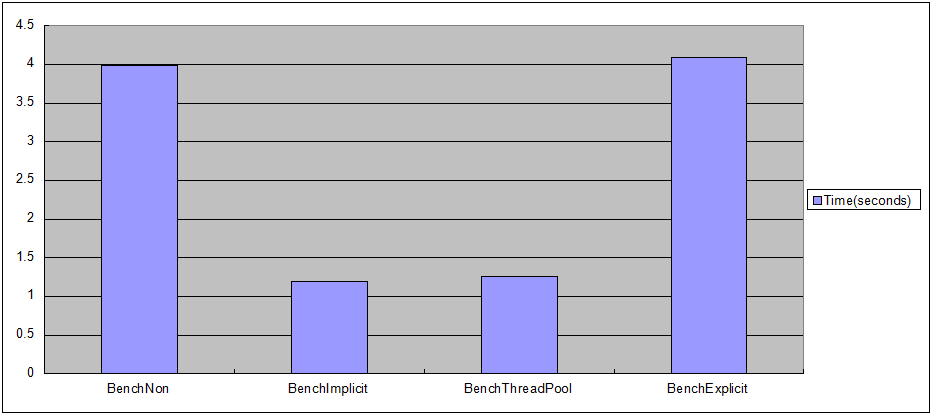
\includegraphics[width=170mm]{benchIntel.png}
\subsubsection{Benchmark test 2}\label{ibt2}
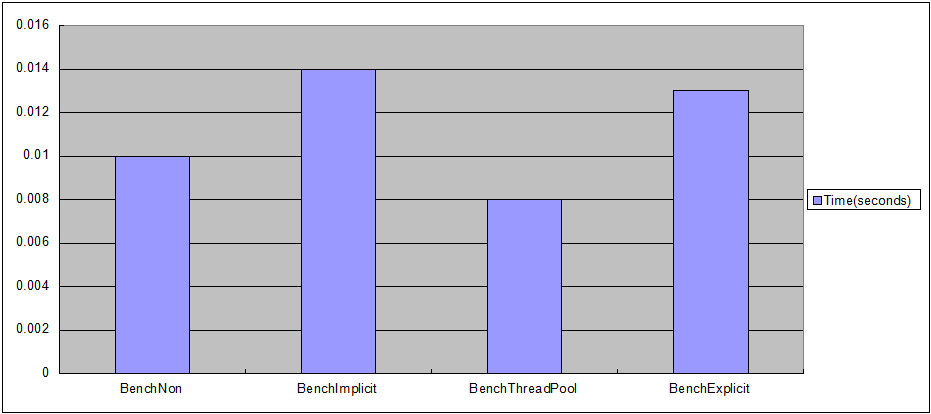
\includegraphics[width=170mm]{benchIntel2.png}

\newpage
\subsection{Benchmark results computer 2}\
All tests for this section were run on a desktop computer which featured an AMD Dual-Core E-300 CPU.\\
\subsubsection{Benchmark test 1}\label{abt1}
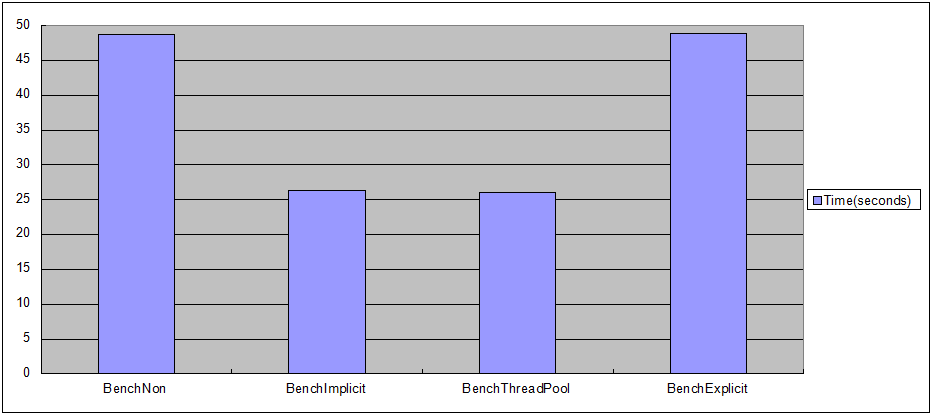
\includegraphics[width=170mm]{benchAMD.png}
\subsubsection{Benchmark test 2}\label{abt1}
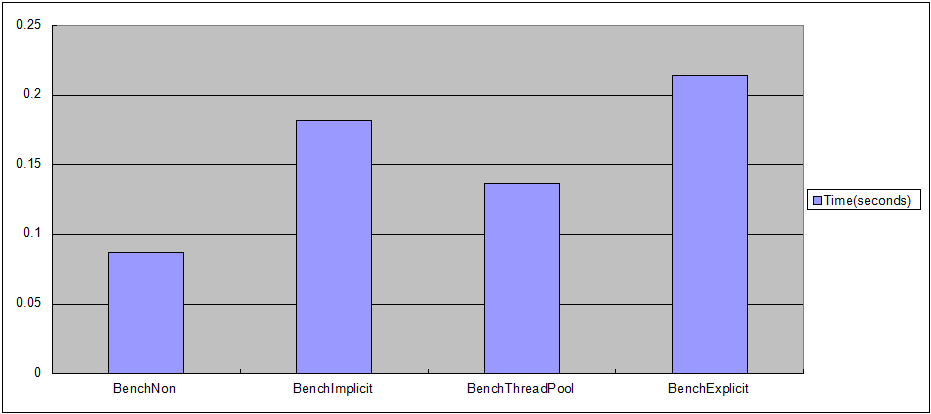
\includegraphics[width=170mm]{benchAMD2.png}

\subsection{Benchmark program classes}\
\subsection{benchmark Class}\
\begin{lstlisting}
import java.util.Random;
import java.util.ArrayList;

/**
 * Created by Chris on 10/12/2015.
 *
 * The main benchmark class for the application is responsible for initializing the
 * various classes and running the tests contained in these classes. It also prints
 * each of the resulting test times.
 */
public class benchMark {

    ArrayList<Integer> arr = new ArrayList<>();
    ArrayList<Integer> arr1 = new ArrayList<>();
    ArrayList<Integer> arr2 = new ArrayList<>();
    ArrayList<Integer> arr3 = new ArrayList<>();
    ArrayList<Integer> arr4 = new ArrayList<>();

    boolean setup = false;

    public benchMark(){

        Random randomGenerator = new Random();
        for (int randNum = 1; randNum <=100000000; ++randNum){
            int randomInt = randomGenerator.nextInt(100);
            arr.add(randomInt);
           
        }

    }
 
    public void bench1(){
        arr.forEach(x -> arr1.add(x));
        benchNon bfl = new benchNon(arr1);
        System.out.println("benchNon test time = " + bfl.test());
        arr1 = null; // Run out of memory if array isn't readied for garbage collection
    }

    public void bench2(){
        arr.forEach(x -> arr2.add(x));
        benchImplicit bIm = new benchImplicit(arr2);
        System.out.println("benchImplicit test time = " + bIm.test());
        arr2 = null;
    }

    public void bench3(){
        arr.forEach(x -> arr3.add(x));
        benchThreadPool btp = new benchThreadPool(arr3);
        System.out.println("benchThreadPool test time = " +btp.test());
        arr3 = null;
    }

    public void bench4(){
        arr.forEach(x -> arr4.add(x));
        benchExplicit bex = new benchExplicit(arr4);
        bex.run();
        while(!bex.complete) {//Make sure both threads have exected before getting result.
        }
        System.out.println("benchExplicit test time = " + bex.result);
        arr4 = null;
    }


    public void runBench(){

        bench1();
        bench2();
        bench3();
        bench4();

    }


    public static void main(String[] args){
        benchMark b = new benchMark();
        b.runBench();
    }
}

\end{lstlisting}
\newpage
\subsubsection{BenchNon Class}\label{benchNon} 
  \begin{lstlisting}
import com.sun.xml.internal.bind.v2.model.annotation.Quick;
import com.sun.xml.internal.fastinfoset.sax.SystemIdResolver;

import java.util.ArrayList;
import java.util.Collections;
import java.util.List;
import java.util.concurrent.TimeUnit;

/**
 * Created by Chris Howell on 10/12/2015.
 *
 * This class takes an ArrayList as an input and then sorts it using the sorter
 * interface default method.
 *
 */
public class benchNon implements sorter{

    List<Integer> arr;

    public benchNon(ArrayList<Integer> arr){

        this.arr = arr;
    }

    /**
     * The test method for this class takes the ArrayList and sorts it before
     * returning the time it took to sort.
     * @return double
     */

    public double test1() {


      long start = System.nanoTime();
      long count=0;
      ;
      // q.sort(arr);
      for(int x = 0; x < arr.size();x++){

          if(isPrime(arr.get(x))) count+=1;

      }

        System.out.println("Total number of prime numbers found=" + count);
        long finish = System.nanoTime();
        double seconds = TimeUnit.MILLISECONDS.convert(finish - start, TimeUnit.NANOSECONDS) / 1000.0;
        return seconds;
    }




}



\end{lstlisting}
\newpage
\subsubsection{BenchImplicit Class}\label{3} 
 \begin{lstlisting}
import java.util.ArrayList;
import java.util.Comparator;
import java.util.List;
import java.util.concurrent.TimeUnit;

/**
 * Created by Chris Howell on 10/12/2015.
 *
 * The benchImplicit Class is the benchmark class that implements a parallel stream
 * to test implicit concurrency.
 *
 * This class takes an ArrayList and uses a parallel stream to sort the ArrayList
 * before returning the times.
 */
public class benchImplicit implements sorter {

    List<Integer> arr = new ArrayList<>();
    public benchImplicit(ArrayList<Integer> arr){
    this.arr = arr;

    }

    public double test1() {

        long start = System.nanoTime();

        long count = arr.parallelStream().filter(x -> (isPrime(x))).count();

        System.out.println("Total number of prime numbers found="+count);
        long finish = System.nanoTime();

        double seconds = TimeUnit.MILLISECONDS.convert(finish - start, TimeUnit.NANOSECONDS) / 1000.0;
        return seconds;
    }



}
\end{lstlisting}

\newpage
\subsubsection{BenchExplicit}\label{thread} 
  \begin{lstlisting}
import java.util.*;
import java.util.concurrent.TimeUnit;

/**
 * Created by Chris on 10/12/2015.
 *
 * This class uses raw threads to count the prime numbers. It works
 * by breaking the array into two separate arrays, and then sequentially
 * checks these two arrays for prime numbers.
 */
class benchExplicit implements Runnable,prime {


    ArrayList<Integer> arr;
    List<Integer> arr1;
    List<Integer> arr2;

    long count = 0;
    public double result;
    public boolean complete = false;

    public benchExplicit(ArrayList<Integer> arr){

        this.arr = arr;
        int  section = arr.size() / 2;

        arr1 = this.arr.subList(0, section);
        arr2 = this.arr.subList(section,section*2);

    }

    public void run() {
        long start = System.nanoTime();
        Thread thread1 = new Thread(new Runnable(){

            @Override
            public void run() {

                for(int x = 0; x < arr1.size();x++){

                    if(isPrime(arr1.get(x))) count+=1;

                }

            }

        });
        thread1.start();
        try {
            thread1.join();// Wait for calculation to finish.
        } catch (InterruptedException e) {
             e.printStackTrace();
        }

        Thread thread2 = new Thread(new Runnable(){

            @Override
            public void run() {

                for(int x = 0; x < arr2.size();x++){

                    if(isPrime(arr2.get(x))) count+=1;

                }

            }

        });
        thread2.start();
        try {
              thread2.join();// Wait for calculation to finish.
        } catch (InterruptedException e) {

            e.printStackTrace();
        }



        long finish = System.nanoTime();
        double seconds = TimeUnit.MILLISECONDS.convert(finish - start, TimeUnit.NANOSECONDS) / 1000.0;

        System.out.println("Total number of prime numbers found=" + count);

        result = seconds;

        complete = true;
    }


}
\end{lstlisting}
 
\newpage
\subsubsection{benchThreadPool}\label{tp} 
  \begin{lstlisting}
import java.util.ArrayList;
import java.util.List;
import java.util.concurrent.*;

/**
 * Created by Chris on 27/02/16.
 *
 * The thread pool class features an inner class which represents the worker
 * thread process for this class. The main thread pool class calculates the
 * number of cores, then generates the appropriate number of threads. Afterwards,
 * it handles the lifetime of a thread while it completes it's operation. A Thread Pool
 * Executor handles the thread creations and execution.
 */
public class benchThreadPool implements prime {

    ArrayList<List<Integer>> arr = new ArrayList<>();

    boolean release = false;
    int cores = Runtime.getRuntime().availableProcessors();
     long count = 0;


    public benchThreadPool(ArrayList<Integer> arr1){
        int  section = arr1.size() / cores;

        int increment = 0;
        int y = 2;


        for(int x = 0; x < cores; x++){

            if(x == 0){
                List<Integer> temp = arr1.subList(increment*section,(section));
                arr.add(temp);
                increment++;
            }
            else{
                List<Integer> temp = arr1.subList(increment*section,section*y);
                arr.add(temp);
                increment++;
                y++;
            }

        }


    }

    public double test(){

        long start = System.nanoTime();

        ThreadPoolExecutor executor = (ThreadPoolExecutor) Executors.newFixedThreadPool(cores);

        List<Future<Long>> results = new ArrayList<>();

        for (int i=0; i<executor.getCorePoolSize(); i++)
        {
            worker work  = new worker(arr.get(i));
            Future<Long> result = executor.submit(work);
            results.add(result);
        }


        for(Future<Long> future : results)
        {
            try
            {
               count += future.get();//Get's the value from the worker, but blocks the thread while it does.
            }
            catch (InterruptedException | ExecutionException e)
            {
                e.printStackTrace();
            }
        }

        executor.shutdown();
        long finish = System.nanoTime();
        double seconds = TimeUnit.MILLISECONDS.convert(finish - start, TimeUnit.NANOSECONDS) / 1000.0;
        System.out.println("Total number of prime numbers found=" + count);
        return seconds;


    }

    class worker implements Callable<Long>
    {

        List<Integer> work;

        public worker(List<Integer> work){


            this.work = work;

        }

        @Override
        public Long call() throws Exception{

            long thisCount =0;

            for(Integer num : work)  if(isPrime(num))  thisCount+=1;

            return thisCount;
        }
    }

}
\end{lstlisting}

\newpage
\subsubsection{Sorter Interface}\label{1} 
  \begin{lstlisting}

/**
 * Created by Chris on 09/03/2016.
 *
 * Interface with default method containing a simple solution to check
 * if a number is a prime number.
 *
 */
public interface prime {

    default boolean isPrime(int n) {
        for(int i=2;i<n;i++) {
            if(n%i==0)return false;
        }
        return true;
    }

}

\end{lstlisting}

\newpage
\subsection{Code examples}
\subsubsection{Synchronized Methods}\label{refSync} 
\begin{lstlisting}
public class ArrayManipulator {

        ArrayList<Integer> arr = new ArrayList<>();

        public synchronized void add(Integer num) {
            arr.add(num);
        }

          public int get(Integer position) {
            return arr.get(position);
        }
    }
\end{lstlisting}

\subsubsection{Lock Example}\label{refLock} 
\begin{lstlisting}
 public void LockExample(){

        ArrayList<Integer> arr = new ArrayList<>();

        arr.add(1);
        arr.add(2);
        arr.add(3);

        Lock lock = new ReentrantLock();

        lock.lock();

        try {
          if(!arr.isEmpty()){
              System.out.println(arr.get(0));
              arr.remove(arr.size()-1);
          }
        } finally {
            lock.unlock();
        }
    }
\end{lstlisting}



\subsubsection{Java Referencing}\label{refExp} 
\begin{lstlisting}
  public void print(){

        ArrayList<Integer> arr1 = new ArrayList<>();

        arr1.add(1);
        arr1.add(2);
        arr1.add(3);

        ArrayList<Integer> arr2 = arr1;

        arr2.add(4);
        System.out.println(arr1.size());//Will print 4

    }
\end{lstlisting} 



\subsubsection{C++ Referencing}\label{refExp2} 
\begin{lstlisting}
    #include <iostream>
    #include <vector>
    using namespace std;
     
    int print() {
    	vector<int> vec; 
    	vec.push_back(1);
    	vec.push_back(2);
    	vec.push_back(3);
    	vector<int> vec2 = vec; 
    	vec2.push_back(1);
    	cout << vec.size() << endl;// Will print 3
       	return 0;
    }
\end{lstlisting} 



\subsubsection{Java Garbage Collection}\label{gc}
\begin{lstlisting}
 public void GarbageCollection(){

        ArrayList<Integer> arr1 = new ArrayList<>();
        
        arr1 = null;//Unused memory will be collected by garbage collector
}
\end{lstlisting} 



\subsubsection{Java Index Out Of Bounds}\label{job} 
\begin{lstlisting}
 public void IndexOutOfBounds(){

        ArrayList<Integer> arr1 = new ArrayList<>();

        arr1.add(1);
        arr1.add(2);
        arr1.add(3);

        int error = arr1.get(4);// Will cause compilation error

        System.out.println(arr1.size());

    }
\end{lstlisting} 

\subsubsection{C++ Error Handling}\label{cob}
\begin{lstlisting}
    #include <iostream>
    #include <vector>
    using namespace std;
     
    int main() {
    	vector<int> vec; 
    	vec.push_back(1);
    	vec.push_back(2);
    	vec.push_back(3);
    	int error = vec[4];
    	cout << vec.size() << endl;// Will print 3
       	return 0;
    }
\end{lstlisting} 

 
 
\end{appendices}



%%%%%%%%%%%%%%%%%%%%%%%%%%%%%%%%%%%%%%%%%
%
%     Bibliography
%
%     Use an easy-to-remember tag for each entry - eg \bibitem{How97} for an article/book by Howie in 1997
%     To cite this publication in your text, write \cite{How97}.  To include more details such as
%     page, Chapter, Theorem numbers, use the form \cite[Theorem 6.3, page 42]{How97}.
%
\begin{thebibliography}{99}

% 
% The usual convention for mathematical bibliographies is to list alphabetically
% by first-named author (then second, third  etc. author then date)
% websites with no author names should go by the site name
%



% Typical layout for reference to a journal article
%
\bibitem{Bovey}
J. D. Bovey, M. M. Dodson,                         % author(s)
The Hausdorff dimension of systems of linear forms % article name
{\em Acta Arithmetica}                             % journal name - italics
{\bf 45}                                           % volume number - bold
(1986), 337--358.                                   % (year), page range

% Typical layout for reference to a website
%
\bibitem{GAP}
The GAP Group, GAP -- Groups, Algorithms, and Programming,  % Site name
Version 4.5.6; 2012. % other information
(http://www.gap-system.org)  % URL


% Typical layout for reference to an online article
%
\bibitem{O_F}
Oracle,                                            % author(s)
{\em Future }, % article name - italics
https://docs.oracle.com/javase/7/docs/api/java/util/concurrent/Future.html % URL
(2004).                                              % (year)
\bibitem{O_P}
Oracle,                                            % author(s)
{\em Parallelism }, % article name - italics
https://docs.oracle.com/javase/tutorial/collections/streams/parallelism.html                       % URL
(2015).                                              % (year)#

% Typical layout for reference to an online article
%
\bibitem{O_F}
Oracle,                                            % author(s)
{\em Future }, % article name - italics
https://docs.oracle.com/javase/7/docs/api/java/util/concurrent/Future.html % URL
(2004).                                              % (year)
\bibitem{O_P}
Ilias\ Koutsakis,                                            % author(s)
{\em java-destructor-why-is-it-missing }, % article name - italics
https://examples.javacodegeeks.com/core-java/java-destructor-why-is-it-missing/ % URL
(2014).                                              % (year)

\end{thebibliography}
\end{document}
\grid
